

\subsubsection{Naručivanje namirnica od snabdevača}


\begin{itemize}
	\item Kratak opis:
		\begin{itemize}
			\item Koordinator proverava status potrebnih namirnica i dogovara narudžbine sa snabdevačima.
		\end{itemize}
	\item Učesnici:
		\begin{itemize}
		    \item Koordinator
		\end{itemize}
	\item Preduslovi:
		\begin{itemize}
		    \item Koordinator je prijavljen na sistem.
		\end{itemize}
	\item Postuslovi:
		\begin{itemize}
			\item Tražene namirnice su poslate.
	\end{itemize}
	\item Osnovni tok:
		\begin{enumerate}
		  % Sistem je sam izracunao za njega sta tacno fali po narudzbinama koje su korisnici izabrali. Onaj slucaj upotrebe koji vrsi magacioner kad stignu namirnice i sistem kad izracuna pokriva pravljenje spiska stvari koje nedostaju
            \item Koordinator pristupa sistemu i bira opciju za proveru stanja namirnica.
           \item Sistem prikazuje koje namirnice nedostaju i količinu koju treba naručiti.
           \item Koordinator bira opciju pretraživanja ponude snabdevača i bira nedostajuće namirnice.
            \item Sistem prikazuje snabdevača čija ponuda pokriva nedostajuće namirnice. 
             \item  Koordinator selektuje snabdevača i unosi porudžbinu namirnica.
              \item Sistem čuva porudžbinu u bazi.
             \item Sistem šalje obaveštenje snabdevaču sa detaljima narudžbine koju treba da pošalje.
            
            
		\end{enumerate}
		\textit{Koraci 3-7 se ponavljaju dokle god postoje namirnice koje nedostaju a nisu poručene.}
	\item Alternativni tok:
		\begin{itemize}
		    \item[2.a] Ukoliko su sve potrebne namirnice dostupne u magacinu slučaj upotrebe se završava.
		 
		\end{itemize}
   \item Dodatne informacije:
		\begin{itemize}
		    \item Podaci o porudžbini podrazumevaju sve namirnice koje su naručene, njihovu količinu, ime snabdevača koji ih dostavlja i vreme isporuke.
	
		\end{itemize}
\end{itemize}

\begin{figure}[H]
\begin{center}
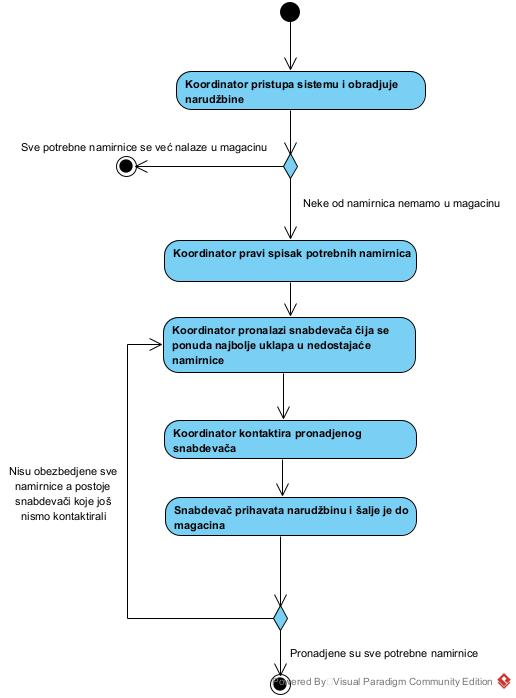
\includegraphics[width=\textwidth]{activity_diagram_order_placment_for_groceries.jpg}
\end{center}
    \caption{Dijagram aktivnosti naručivanja namirnica od snabdevača}
\label{fig:Activity_diagram_order_placment_for_groceries}
\end{figure}
